\begin{figure}[h]
	\centering	
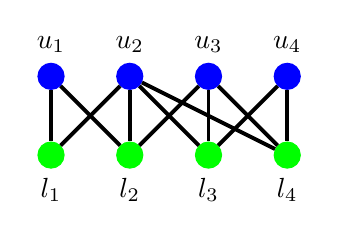
\begin{tikzpicture}
 \node[shape=circle,draw=blue,fill=blue,label=above:$u_1$] (u1) {};
 \node[shape=circle,draw=blue,fill=blue,label=above:$u_2$] (u2) [right of=u1] {};
 \node[shape=circle,draw=blue,fill=blue,label=above:$u_3$] (u3) [right of=u2] {};
 \node[shape=circle,draw=blue,fill=blue,label=above:$u_4$] (u4) [right of=u3] {};
 \node[shape=circle,draw=green,fill=green,label=below:$l_1$] (l1) [below of=u1] {};
 \node[shape=circle,draw=green,fill=green,label=below:$l_2$] (l2) [below of=u2] {};
 \node[shape=circle,draw=green,fill=green,label=below:$l_3$] (l3) [below of=u3] {};
 \node[shape=circle,draw=green,fill=green,label=below:$l_4$] (l4) [below of=u4] {};

 \draw (u1) [line width=0.5mm] -- (l1);
 \draw (u1) [line width=0.5mm] -- (l2);
 \draw (u2) [line width=0.5mm] -- (l1);
 \draw (u2) [line width=0.5mm] -- (l2);
 \draw (u2) [line width=0.5mm] -- (l3);
 \draw (u2) [line width=0.5mm] -- (l4);
 \draw (u3) [line width=0.5mm] -- (l2);
 \draw (u3) [line width=0.5mm] -- (l3);
 \draw (u3) [line width=0.5mm] -- (l4);
 \draw (u4) [line width=0.5mm] -- (l3);
 \draw (u4) [line width=0.5mm] -- (l4);
\end{tikzpicture}

\caption{Example of \acrshort{bg}}
\label{fig:bipartite-graph-example}
\end{figure}

 